\documentclass{beamer}
\usepackage[utf8]{inputenc}

\usepackage[utf8]{inputenc}
\usepackage[T1]{fontenc}

\usepackage[english]{babel}
\usepackage{amsmath}
\usepackage{cleveref}
\usepackage{amssymb}
\usepackage{mathtools}

%%Numbers, expectation
\newcommand{\N}{\mathbb{N}}
\newcommand{\E}{\mathbb{E}}
\renewcommand{\P}{\mathbb{P}}
\newcommand{\Var}{\mathbb{V}}
\newcommand{\R}{\mathbb{R}}
\newcommand{\D}{\mathcal{D}}
\newcommand{\B}{\mathcal{B}}
\newcommand{\Dh}{\D_h}
\renewcommand{\phi}{\varphi}
\newcommand*\diff{\mathop{}\!\mathrm{d}} % integral

%% mathoperator
\DeclareMathOperator*{\argmax}{arg\,max}
\DeclareMathOperator*{\argmin}{arg\,min}
\DeclareMathOperator*{\dom}{dom}
\DeclareMathOperator*{\sign}{sign}
\DeclareMathOperator*{\diag}{diag}

\DeclareMathOperator*{\Cov}{Cov}
\DeclareMathOperator*{\Cor}{Corr}
\DeclareMathOperator*{\Id}{Id}

%proximal operator
\newcommand{\prox}[3][]{\operatorname{prox}^{#1}_{#2}\left(#3 \right)}

\usepackage{xcolor}

%% sort citations by increasing number
\usepackage[sort,nocompress]{cite}

\usepackage{graphicx}% http://ctan.org/pkg/graphicx
\graphicspath{{../figures/}{../../figures}{../../memes}} %Setting the graphicspath
\usepackage{caption,subcaption}

\usepackage{tikz}
\usepackage{pgfplots}
\usetikzlibrary{backgrounds}
\usetikzlibrary{intersections}
\usepgfplotslibrary{fillbetween}

% \usepackage[right]{showlabels}


%%
\theoremstyle{plain}
\newtheorem{prop}{Proposition}[section]
\newtheorem{algo}{Algorithm}[section]
\newtheorem{assumption}{Assumption}
\theoremstyle{remark}
\newtheorem{remark}{Remark}[section]

% cref
\crefname{assumption}{Assumption}{Assumptions}
\crefname{equation}{}{}

\usepackage{autonum}

\usepackage{bm} %% bold math symbols

\usepackage{bbm} %% for \mathbbm{1}


% algorithmic environment
\usepackage{algorithm}
\usepackage[noend]{algpseudocode}

% for some reason this was required on one void linux installation (but not the other)
\usepackage{sansmathaccent}
\pdfmapfile{+sansmathaccent.map}

\author{Axel Böhm}

% shows which section we're in
\usetheme{Darmstadt}

% page number
\setbeamertemplate{footline}[frame number]
\setbeamercolor{page number in head/foot}{fg=gray}


% display things like onslide or visible already before but grayed out
\setbeamercovered{transparent}

% set the itemize item symbol as a diamond
\setbeamertemplate{itemize item}{$\diamond$}
% set the itemize subitem symbol as a triangle
\setbeamertemplate{itemize subitem}{$\blacktriangleright$}

% set the enumerate item symbol as a roman numbers
\setbeamertemplate{enumerate item}{(\roman{enumi})}


\author{Axel Böhm}

% shows which section we're in
\usetheme{Darmstadt}

% page number
\setbeamertemplate{footline}[frame number]
\setbeamercolor{page number in head/foot}{fg=gray}


% display things like onslide or visible already before but grayed out
\setbeamercovered{transparent}

% set the itemize item symbol as a diamond
\setbeamertemplate{itemize item}{$\diamond$}
% set the itemize subitem symbol as a triangle
\setbeamertemplate{itemize subitem}{$\blacktriangleright$}

% set the enumerate item symbol as a roman numbers
\setbeamertemplate{enumerate item}{(\roman{enumi})}


\newcounter{sauvegardeenumi}
\newcommand{\asuivre}{\setcounter{sauvegardeenumi}{\theenumi}}
\newcommand{\suite}{\setcounter{enumi}{\thesauvegardeenumi}}

\title{Mirror Descent}
\date{\today}

\begin{document}
\maketitle
\frame{\tableofcontents}

\section{About norms}

\begin{frame}
  \frametitle{Recap on (sub)-gradient descent}

  \begin{itemize}
    \item When we used a norm $\Vert \cdot \Vert$ we meant the \emph{$2$-norm}, i.e.\
          \begin{equation}
            \Vert x \Vert_2 = \sqrt{x_1^2 + x_2^2 + \dots + x_d^2 }. %{\Big({\sum_{i=1}^{d} x_i^2} \Big)}^{1/2}.
          \end{equation}
    \item In \textbf{gradient descent} we used Lipschitz continuity:
          \begin{equation}
            \Vert \nabla f(x) - \nabla f(y) \Vert \le L \Vert x-y \Vert.
          \end{equation}
          (Lead to a complexity of $\mathcal{O}(\frac{L}{k})$) \\

    \item \textbf{Sub-gradient descent}: used $\Vert g \Vert \le G$ which lead to $\mathcal{O}(\frac{G}{\sqrt{k}})$.

  \onslide<2->{%
    \item But there are \textcolor{blue}{other norms} $\Vert x \Vert_\infty \le \Vert x \Vert_2 \le \sqrt{d} \Vert x \Vert_\infty$.\\

    It can happen that $  \Vert g \Vert_\infty \le G \quad \text{but} \quad \Vert g \Vert_2 \approx \sqrt{d}G$.
          \begin{block}{}
            \begin{center}
              we lose dimension independence
            \end{center}

          \end{block}
  }
  \end{itemize}
\end{frame}


\begin{frame}
  \frametitle{Different norms?}
  \begin{center}
    \textit{But where did we use the norm in the \textbf{method}?}
  \end{center}

  \begin{block}{Gradient Descent}
    \begin{equation}
      x_{k+1} = x_k - \alpha \nabla f(x_k)
    \end{equation}
    equivalently
    \begin{equation}
      x_{k+1} = \argmin_{x \in \R^d} \left\{ f(x_k) + \langle \nabla f(x_k), x-x_k \rangle + \frac{1}{2 \alpha} \Vert x-x_k  \Vert_2^2 \right\}
    \end{equation}
  \end{block}
  We can replace the $2$-norm with a more general \textbf{distance}.
\end{frame}


\section{Bregman distances}%

\begin{frame}
  \frametitle{Bregman distance}
  $h: \R^d \to \R \cup \{+\infty\}$ is convex
  \begin{enumerate}
    \item h is differentiable of the interior of $\dom h$
    \item h is $1$-strongly convex w.r.t. $\Vert \cdot \Vert_2$
  \end{enumerate}
  Then
  \begin{equation}
    \Dh(x,y) := h(x) - h(y) - \langle \nabla h(y), x-y \rangle.
  \end{equation}

  \onslide<2->{%
    \begin{block}{Properties}
      \begin{itemize}
        \item $\Dh(x, y) \ge 0$
        \item $\Dh(x, y) \neq \Dh(y, x)$
        \item $\Dh(\cdot, y)$ is convex for all $y$
              \begin{equation}
                \Dh(x,y) \approx \frac12 \langle \nabla^2h(y)(x-y), x-y \rangle = \frac12 \Vert x-y \Vert_{\nabla^2h(y)}^2
              \end{equation}
        \item $\Dh(x, y) \ge \frac12 \Vert x-y \Vert^2$ ($1$-strong convexity)
      \end{itemize}
    \end{block}
  }
\end{frame}


\begin{frame}
  \frametitle{Examples} % of Bregman distances
  \begin{itemize}
    \item $h(x) = \frac12 \Vert x \Vert_2^2$ gives $\Dh(x,y) = \Vert x-y \Vert^2$
    \item $h(x) = \frac{1}{2(p-1)} \Vert x \Vert_p^2$ with $p \in [1, 2]$
    \item  $\Delta^d= \{x \in \R^d_+ : \sum_{i=1}^{d}x_i = 1\}$ the \emph{unit simplex} and
          \begin{equation}
            h(x) =
            \begin{cases}
              \sum_{i=1}^{d} x_i \log(x_i) & x_i > 0 \\
              +\infty & \text{otherwise}
            \end{cases}
          \end{equation}
          the \textbf{Negative entropy}.\\
  \end{itemize}
\end{frame}


\begin{frame}
  \frametitle{Negative entropy}
  \begin{itemize}
    \item Negative entropy: $h(x) = \sum_{i=1}^{d} x_i \log(x_i)$ for $ x_i > 0$. \\
    \item Then $ \nabla h(x) = \log(x) + \bm{1}$ (coordinatewise) and
    \begin{equation}
    \begin{aligned}
        \Dh(x,y) &= \sum_{i=1}^{d}x_i \log(x_i) - y_i \log(y_i) - \langle \log(y)+ \bm{1}, x-y \rangle \\
        &= \sum_{i=1}^{d} x_i \log(x_i) - \sum_{i=1}^{d} x_i \log(y_i) \\
        &= \sum_{i=1}^{d} x_i \log\left(\frac{x_i}{y_i}\right)
    \end{aligned}
    \end{equation}
    Known as \textcolor{blue}{Kullback-Leibler divergence} $K(X \Vert Y)$.
    \item Is strongly convex over $\Delta$
    \begin{equation}
      \D(x, y) \ge \frac12 \Vert x-y \Vert_1^2 \quad \text{Pinsker's ineq.}
    \end{equation}
  \end{itemize}
\end{frame}


\section{Mirror descent}%

\begin{frame}
  \frametitle{Mirror descent}
    Idea: replace squared Euclidian norm with more general object:
    \begin{equation}
      \begin{aligned}
        x_{k+1} &= \argmin_{x \in \R^d} \{ f(x_k) + \langle \nabla f(x_k), x-x_k \rangle + \frac{1}{\alpha} \Dh(x,x_k)\} \\
        \onslide<2->{%
          &= \argmin_{x \in \R^d} \{ \langle \nabla f(x_k), x \rangle + \frac{1}{\alpha} \Dh(x,x_k)\} \\
          &= \argmin_{x \in \R^d} \{ \langle \nabla f(x_k), x \rangle + \frac{1}{\alpha} (h(x) - h(x_k) - \langle \nabla h(x_k), x-x_k \rangle)\} \\
          &= \argmin_{x \in \R^d} \{ \langle \nabla f(x_k), x \rangle + \frac{1}{\alpha} (h(x) - \langle \nabla h(x_k), x \rangle)\} \\
          &= \argmin_{x\in \R^d} \{ \langle \alpha \nabla f(x_k) - \nabla h(x_k), x \rangle + h(x) \} \\
        }
      \end{aligned}
    \end{equation}

    \onslide<3->{%
      \textbf{Question:} But why \emph{mirror} descent?
    }
\end{frame}


\begin{frame}
  \frametitle{The Mirror part}
  \begin{equation}
    x_{k+1} = \argmin_{x\in \R^d} \{ \langle \alpha \nabla f(x_k) - \nabla h(x_k), x \rangle + h(x) \}
  \end{equation}
  By optimality condition:
  \begin{equation}
    0 = \alpha \nabla f(x_k) - \nabla h(x_k) + \nabla h(x_{k+1})
  \end{equation}
  Therefore
  \begin{equation}
    \nabla h(x_{k+1}) =  \nabla h(x_k)  - \alpha \nabla f(x_k)
  \end{equation}
\end{frame}


\begin{frame}
  \frametitle{Why it's called mirror descent}
  \begin{figure}[ht]
    \centering
    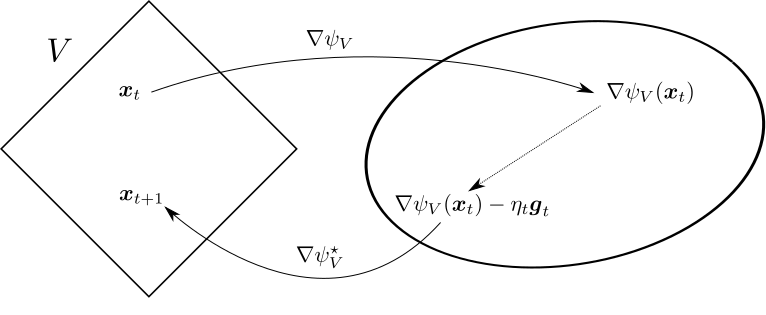
\includegraphics[width=\textwidth,height=\textheight,keepaspectratio]{mirror}
    \caption{$\psi = h$}
  \end{figure}
\end{frame}

% yura mirror descent part 2 begins here

\begin{frame}
  \frametitle{Mirror Descent w.r.t. negative entropy}
    \textcolor{blue}{Negative entropy}: $h(x) = \sum_{i=1}^{d} x_i \log(x_i)$ for $ x_i > 0$. \\
    We define $a := \alpha \nabla f(x_k) - \nabla h(x_k)$. Then
    \begin{equation}
      x_{k+1} = \argmin_{x \in \Delta} \{ \langle a, x \rangle + h(x)\}
    \end{equation}
    Results in
    \begin{equation}
      x_{k+1} = x_k .* e^{- \alpha \nabla f(x_k)}
    \end{equation}
    in a pointwise sense.
\end{frame}


% includes bregman projections which I didn't plan on covering

% \begin{frame}
%   \frametitle{Mirror Descent on the unit simplex}
%     \textcolor{blue}{Negative entropy}: $h(x) = \sum_{i=1}^{d} x_i \log(x_i)$ for $ x_i > 0$. \\
%     We define $a := \alpha \nabla f(x_k) - \nabla h(x_k)$. Then
%     \begin{equation}
%       x_{k+1} = \argmin_{x \in \Delta} \{ \langle a, x \rangle + h(x)\}
%     \end{equation}
%     with $x_i \ge 0$ and $\sum x_i = 1$.
%     \begin{block}{How to solve this?}
%       Via \textbf{Lagrange }
%       \begin{equation}
%         L(x,\mu) = \langle a, x \rangle + h(x) - \mu (x_1+\cdots+ x_d -1)
%       \end{equation}
%     \end{block}
% \end{frame}
% \begin{frame}
%   \frametitle{Mirror Descent on the unit simplex [contd]}
%       Then,
%       \begin{equation}
%         \begin{aligned}
%           \partial_{x_i} L(x,\mu) &= a_i + \log(x_i) +1 - \mu \overset{!}{=} 0 \\
%           \log(x_i) &= \mu -1 - a_i  \\
%           x_i &= e^{\mu - 1 - a_i} = \beta e^{-a_i}
%         \end{aligned}
%       \end{equation}
%       with $\beta= e^{\mu-1}$.

%       \onslide<2->{%
%         Second constraint:
%         \begin{equation}
%           \begin{aligned}
%             \sum_{i=1}^{d} x_i \overset{!}{=} 1
%             &\Rightarrow \sum_{i=1}^{d} \beta e^{-a_i} = 1
%             \Rightarrow \beta = \frac{1}{\sum_{i=1}^{d} e^{-a_i}} \Rightarrow x_i = \frac{e^{-a_i}}{\sum_{j=1}^{d} e^{-a_j}}
%           \end{aligned}
%         \end{equation}
%       }

%       \onslide<3->{%
%         Final mirror descent update:
%         \begin{equation}
%           x_{k+1}(i) = \frac{x_k(i) e^{\alpha {[\nabla f(x_k)]}_i}}{\sum_{j=1}^{d}e^{\alpha {[\nabla f(x_k)]}_j}}
%         \end{equation}
%       }
% \end{frame}


\begin{frame}
  \frametitle{(General) mirror descent convergence statement}
  Since we changed norm in the space of the variable $x$, we need to go to the \textcolor{blue}{dual norms} in the space of the subgradients
  \begin{equation}
    \Vert y \Vert_* := \max_{\Vert x \Vert=1} \{ \langle y, x \rangle\}.
  \end{equation}
  \begin{theorem}
    In $(\R^d, \Vert \cdot \Vert)$ and subgradients bounded in dual norm $\Vert g_k \Vert_* \le G$, then
    \begin{equation}
      f(\bar{x}_k) - f^* \le \frac{{(\D(x^*, x_0))}^{1/2} G}{\sqrt{k}},
    \end{equation}
    where $\bar{x}_k$ denotes the averaged iterates, as usual.
  \end{theorem}
\end{frame}


\begin{frame}
  \frametitle{Convergence w.r.t. negative entropy}
    It might occur that
    \begin{equation}
      \Vert g \Vert_\infty = (\Vert g \Vert_1)_* \le G
    \end{equation}
    but
    \begin{equation}
      \Vert g \Vert_2 \approx \sqrt{d} G.
    \end{equation}
    But is are all the bounds of the previous theorem dimension independent?\\
    \textbf{What about $\D(x^*, x_0) $?}
    Let $x_0 = (\frac{1}{n}, \cdots , \frac{1}{n})$, then
    \begin{equation}
      \D(x, x_0) = \sum x_i \log\left(\frac{x_i}{\frac1n}\right) = \sum x_i \log(x_i) + \log(n) \le \log(n)
    \end{equation}
    while $ \Vert x_0 - x^* \Vert^2 \le 2$.

\end{frame}


\begin{frame}
  \frametitle{Proof}
  In the Euclidian space we used
  \begin{align}
    \MoveEqLeft \langle x_{k+1}-x_k, x^* -x_{k+1} \rangle \\
    &= \frac12 \Vert x^*-x_k \Vert^2 - \frac12 \Vert x^*-x_{k+1} \Vert^2 - \frac12 \Vert x_{k+1}-x_k \Vert^2.
  \end{align}
  Similar \textcolor{blue}{$3$-point identity} holds for Bregman distances:
  \begin{align}
    \MoveEqLeft \langle \nabla h(x_{k+1})-\nabla h(x_k), x^*-x_{k+1} \rangle =\\
    &= D(x^*, x_k) - D(x^*, x_{k+1}) - D(x_{k+1}, x_k).
  \end{align}
  Therefore
  \begin{equation}
    D(x^*, x_{k+1}) \le  D(x^*, x_k) - D(x_{k+1}, x_k) + \alpha \langle g_k, x^*-x_{k+1} \rangle.
  \end{equation}
\end{frame}


\begin{frame}
  \frametitle{Proof II}
  \begin{equation}
    D(x^*, x_{k+1}) \le  D(x^*, x_k) - D(x_{k+1}, x_k) + \alpha \langle g_k, x^*-x_{k+1} \rangle.
  \end{equation}
  Last term is not quite right.
  \begin{align}
    \langle g_k, x^*-x_{k+1} \rangle &= \langle g_k, x^*-x_k \rangle + \langle g_k, x_k-x_{k+1} \rangle \\
                         &\le f(x^*)-f(x_k) + \Vert g_k \Vert_* \Vert x_k-x_{k+1} \Vert \\
    &\le f(x^*)-f(x_k) + \frac{\alpha \Vert g_k \Vert_*^2}{2} + \frac{\Vert x_k-x_{k+1} \Vert^2}{2 \alpha}.
  \end{align}
  Combined we get that
  \begin{align}
    D(x^*, x_{k+1}) &\le  D(x^*, x_k) - D(x_{k+1}, x_k) + \alpha (f(x^*)-f(x_k)) \\
    &\quad+ \frac{\alpha^2 \Vert g_k \Vert_*^2}{2} + \frac{\Vert x_k-x_{k+1} \Vert^2}{2}.
  \end{align}
\end{frame}


\begin{frame}
  \frametitle{Proof III}
  We assumed strong convexity of $h$:
  \begin{align}
    D(x_{k+1}, x_k) \ge \frac12 \Vert x_{k+1}-x_k \Vert^2.
  \end{align}
  Yields
  \begin{align}
    D(x^*, x_{k+1}) \le  D(x^*, x_k) + \alpha (f(x^*)-f(x_k))  + \frac{\alpha^2 \Vert g_k \Vert_*^2}{2} \\
  \end{align}
  Continue as always
  \begin{align}
    \frac{1}{k} \sum_{i=1}^{k} f(x_i) - f^* \le \frac{D(x^*, x_0)}{\alpha k}
    \frac{\alpha G^2}{2} \\
  \end{align}
\end{frame}


\begin{frame}
  \frametitle{What about the smooth case}

  \begin{itemize}
    \item Talked about how to get better constants in the ``bounded subgradients'' setting
    \item but can't make them bounded if they are not
  \end{itemize}
  However,
  \begin{itemize}
    \item Can also come up with a new notion of smoothness
          \begin{align}
            f(y) \le f(x) + \langle \nabla f(x), y-x \rangle + L D(y, x)
          \end{align}
    \item which might hold even if $f$ is not smooth in classical sense
  \end{itemize}
\end{frame}

\end{document}
